\documentclass[sigconf]{acmart}

% Recommended, but optional, packages for figures and better typesetting:
\usepackage{microtype}
\usepackage{graphicx}
%\usepackage{subfigure}
\usepackage{booktabs} % for professional tables
\usepackage{hyperref}

% Attempt to make hyperref and algorithmic work together better:
\newcommand{\theHalgorithm}{\arabic{algorithm}}

% additional packages
%\usepackage[numbers,compress]{natbib}
\usepackage{mathtools}
\usepackage{amsfonts}
\usepackage{amsmath,amssymb}%,amsthm}
\usepackage{mathrsfs}
\usepackage{nicefrac}  % compact symbols for \nicefrac[]{1}{2}, etc.
%\usepackage[table]{xcolor} % colour table

\usepackage{bm}
\usepackage{bbm}
\usepackage{stmaryrd}
\usepackage{enumerate}
\usepackage{algorithm}
\usepackage{algorithmic}
\usepackage{tablefootnote}    % footnote in table and tabular env
\usepackage{footmisc}   % \footref, refer the same footnote at different places
\usepackage{subcaption} % sub-figures, cannot be used with subfigure package
\usepackage{setspace}   % set space between lines
\usepackage[english]{babel}
\usepackage{multirow} % for tables
\usepackage{colortbl} % cellcolor
\graphicspath{{fig/}}   % Location of the graphics files

%\newtheorem{theorem}{Theorem}
%\newtheorem{corollary}{Corollary}
%\newtheorem{lemma}{Lemma}
%\newtheorem{proposition}{Proposition}
%\newtheorem{remark}{Remark}

\DeclareMathOperator*{\argmin}{argmin}
\DeclareMathOperator*{\argmax}{argmax}
\newcommand{\eat}[1]{}
\newcommand{\given}{\mid}
\newcommand{\llb}{\llbracket}
\newcommand{\rrb}{\rrbracket}
\newcommand{\bu}{\mathbf{u}}
\newcommand{\bv}{\mathbf{v}}
\newcommand{\bb}{\mathbf{b}}
\newcommand{\bc}{\mathbf{c}}
\newcommand{\f}{\mathbf{f}}
\newcommand{\h}{\mathbf{h}}
\newcommand{\x}{\mathbf{x}}
\newcommand{\y}{\mathbf{y}}
\newcommand{\z}{\mathbf{z}}
%\newcommand{\1}{\mathbf{1}}
\newcommand{\w}{\mathbf{w}}
\newcommand{\A}{\mathbf{A}}
\newcommand{\B}{\mathbf{B}}
%\newcommand{\C}{\mathbf{C}}
\newcommand{\D}{\mathbf{D}}
%\newcommand{\G}{\mathbf{G}}
\newcommand{\I}{\mathbf{I}}
\newcommand{\Hb}{\mathbf{H}}
\newcommand{\M}{\mathbf{M}}
\newcommand{\Pb}{\mathbf{P}}
\newcommand{\Q}{\mathbf{Q}}
\newcommand{\W}{\mathbf{W}}
\newcommand{\V}{\mathbf{V}}
\newcommand{\X}{\mathbf{X}}
\newcommand{\Y}{\mathbf{Y}}
\newcommand{\Z}{\mathbf{Z}}
\newcommand{\p}{\mathbb{P}}
\newcommand{\E}{\mathbb{E}}
\newcommand{\R}{\mathbb{R}}
\newcommand{\q}{\mathbf{q}}
\newcommand{\DCal}{\mathcal{D}}
\newcommand{\LCal}{\mathcal{L}}
\newcommand{\RCal}{\mathcal{R}}
\newcommand{\SCal}{\mathcal{S}}
\newcommand{\XCal}{\mathcal{X}}
\newcommand{\YCal}{\mathcal{Y}}
\newcommand{\WCal}{\mathcal{W}}
\newcommand{\alphat}{\widetilde{\alpha}}
\newcommand{\betat}{\widetilde{\beta}}
\newcommand{\gammat}{\widetilde{\gamma}}
\newcommand{\phit}{\widetilde{\phi}}
\newcommand{\bt}{\widetilde{b}}
\newcommand{\alphabm}{{\bm{\alpha}}}
\newcommand{\betabm}{{\bm{\beta}}}
\newcommand{\gammabm}{{\bm{\gamma}}}
\newcommand{\deltabm}{{\bm{\delta}}}
\newcommand{\bmu}{\bm{\mu}}
\newcommand{\nubm}{\bm{\nu}}
\newcommand{\phibm}{\bm{\phi}}
\newcommand{\xibm}{\bm{\xi}}
\newcommand{\thetabm}{\bm{\theta}}
\newcommand{\Thetabm}{\mathbf{\Theta}}
\newcommand{\lambdabm}{\bm{\lambda}}
\newcommand{\Lambdabm}{\mathbf{\Lambda}}
\newcommand{\Omegabm}{\bm{\Omega}}
\newcommand{\Phibm}{\mathbf{\Phi}}
\newcommand{\one}{\mathbf{1}}
\newcommand{\zero}{\mathbf{0}}
\newcommand{\equiva}{\Leftrightarrow}
%\newcommand{\widebar}[1]{\mkern 1.5mu\overline{\mkern-1.5mu#1\mkern-1.5mu}\mkern 1.5mu}
%\newcommand{\widebar}[1]{\mkern 1.5mu\overline{\mkern-1.5mu#1\mkern-2.5mu}\mkern 3mu}
\newcommand{\widebar}[1]{\mkern 1.5mu\overline{\mkern-2.5mu#1\mkern-1.5mu}\mkern 1.5mu}

% madeness: suPer-script in Brackets
\newcommand{\pb}[1]{^{({#1})}}
\newcommand{\eg}{e.g.,\ }
\newcommand{\ie}{i.e.,\ }
\newcommand{\diag}{\text{diag}}
\newcommand{\downto}{\,\textbf{downto}\,}
\newcommand{\blue}[1]{{\color{blue}{#1}}}
\newcommand{\green}[1]{{\color{green}{#1}}}
\newcommand{\firstBest}[1]{\cellcolor{gray!50}{#1}}
\newcommand{\secondBest}[1]{\cellcolor{yellow!20}{#1}}

\newcommand{\TODO}{\blue{\bf{TODO:\ }}}
\newcommand{\DONE}{\green{\bf{DONE\ }}}
\newcommand{\cheng}[1]{\color{magenta}{\bf{Cheng:\ #1}}\color{black}}


% Copyright
%\setcopyright{none}
%\setcopyright{acmcopyright}
%\setcopyright{acmlicensed}
\setcopyright{rightsretained}
%\setcopyright{usgov}
%\setcopyright{usgovmixed}
%\setcopyright{cagov}
%\setcopyright{cagovmixed}


% DOI
%\acmDOI{10.475/123_4}

% ISBN
%\acmISBN{123-4567-24-567/08/06}

%Conference
\acmConference[RecSys'18]{ACM Conference on Recommender Systems}{October 2-7, 2018}{Vancouver, Canada}
\acmYear{2018}
\copyrightyear{2018}
%\acmArticle{4}
%\acmPrice{15.00}

% Remove the non-mandatory "ACM Reference format."
\fancyhead{}
\settopmatter{printacmref=false, printfolios=false}

\allowdisplaybreaks


\begin{document}
%\title{Music recommendation and playlist augmentation using multitask classification and ranking}
%\title{Augment Music Playlist via Multitask Classification and Ranking}
%\title{Music Recommendation via Multitask Learning}
%\title{Multitask Learning for Cold-Start Music Recommendation}
%\title{Cold-start Music Recommendation via Multitask Learning}
\title{Cold-start Playlist Recommendation via Multitask Learning}

%\author{Author Name}
%\affiliation{\institution{Institution Name}}
%\email{Email Address}

% The default list of authors is too long for headers.
%\renewcommand{\shortauthors}{B. Trovato et al.}

%
% The code below should be generated by the tool at
% http://dl.acm.org/ccs.cfm
% Please copy and paste the code instead of the example below.
%

\keywords{Playlist recommendation, Cold start, Multitask learning}

\begin{abstract}
% !TEX root=./main.tex

%Playlists are a core feature of music streaming services.
Playlist recommendation concerns producing a sequence of songs that a user might enjoy.
We investigate this problem in three different cold-start scenarios:
%Specifically, we investigate three settings with different cold items:
(i) \emph{cold playlists}, where we recommend a set of songs to form a new playlist for an existing user; %without additional context except the user;
(ii) \emph{cold songs}, where we recommend newly released songs to extend existing playlists;
(iii) \emph{cold users}, where we recommend a set of songs to form a new playlist for a new user. %, without any other context.
%
We propose a flexible multitask learning method to deal with all three settings.
The method learns from user-curated playlists,
%the %multitask learning
%method
and encourages songs in the playlist 
to be ranked higher than those are not
by minimising a %the Bottom-Push
bipartite ranking loss.
We formulate the objective as a constrained convex optimisation problem,
and show how this may be approximated by an unconstrained objective
%then address the difficulty of a large number of constraints by approximating the %Bottom-Push loss
%bipartite ranking loss
%with a classification loss
inspired by an equivalence relationship between bipartite ranking and binary classification.
Empirical results on two real music playlist datasets show the proposed approach has good performance for playlist recommendation
in cold-start settings.
%in three cold-start settings.

\end{abstract}

\maketitle

% !TEX root=./main.tex

\section{Introduction}
\label{sec:intro}
Online music streaming services (e.g., Spotify, Pandora, Apple Music) % Google Play Music, Amazon Music) 
play an increasingly important role in the digital music industry.
A key ingredient of these services is the ability to automatically recommend songs to help users explore large collections of music.
%as well as create an uninterrupted listening experience.
Such recommendation is often in the form of a \emph{playlist}, 
%which is simply an ordered sequence of songs
which involves a (small) set of songs.
%
% one paragraph about recommender system
Conventional recommender systems for books or movies~\citep{Sarwar:2001,Netflix}
typically learn a score function via matrix factorisation~\citep{Koren:2009},
and recommend the item that achieves the highest score.
This approach is not suited to %deal with 
\emph{cold-start} settings,
where there is no historical data for either users or items.
%
% explain what is different about recommending playlist
Further, in playlist recommendation,
one has to recommend a subset of a large collection of songs instead of only one top ranked song.
Enumerating all possible such subsets is intractable;
additionally,
it is likely that more than one playlist is satisfactory, since
users generally maintain more than one playlist when using a music streaming service,
which leads to challenges in standard supervised learning.


%We investigate the problem of recommending a playlist of songs for a given user.
%If the user is new to the system, we would like to make a decent default recommendation by learning from 
%all available playlists of existing users.
%On the other hand, if the user already has a few playlists in the system, it is expected the recommender 
%system can also learn from this information and hopefully make better recommendations.
%
We investigate the problem of recommending songs to form personalised playlists %(for a given user)
in cold-start settings by learning from user-curated playlists.
%
%First, we study the problem of recommending a set of songs to form a playlist for a new user (\ie \emph{cold user}).
%We find it is challenging to improve recommendations beyond simply ranking songs according to their popularity,
%which is consistent with discoveries in~\cite{mcfee2012million,bonnin2013evaluating,bonnin2015automated}.
% the reason is believed to be that a small number of popular songs appeared in a large number of playlists, 
% and the majority of songs only appear in a few playlists~\cite{bonnin2013evaluating}.
% This is consistent with discoveries in~\cite{bonnin2013evaluating,jannach2015beyond,bonnin2015automated}
%
First, we study the problem of recommending a set of songs to form a new playlist for a user
%We learn the preference of the given user from her existing playlists,
by exploiting the (implicit) preference %of the given user 
from her existing playlists.
We find that learning from a user's existing playlists %can significantly 
improves the accuracy of recommendation.
Since we do not have any contextual information about the new playlist, 
we call this setting \emph{cold playlists}.
%
We further consider the setting of new users (\ie \emph{cold users}),
where we recommend playlists for new users.
We find it challenging to improve recommendations beyond simply ranking songs according to their popularity 
if we know nothing about the user, which is consistent with previous 
discoveries~\cite{mcfee2012million,bonnin2013evaluating,bonnin2015automated}.
However, improvement can still be achieved if we know a few simple attributes (\eg age, gender, country etc.)
of the users.
%
%This motivates us to exploit the (implicit) user preference from her existing playlists,
%which leads to the \emph{cold playlists} setting,
%where a set of songs are recommended to form a new playlist for an existing user. %of a music service.
%We find that learning from a user's existing playlists %can significantly 
%improves the accuracy of recommendation.
%
%In addition, 
%We further investigate the value of seed songs for improving recommendation.
%This results in the \emph{cold songs} setting,
%where we recommend a set of newly released songs to extend users' existing playlists. %from users.
%
Lastly, we investigate the problem of recommending newly released songs (\ie \emph{cold songs}) to extend users' existing playlists. 
We find that songs in a playlist are especially helpful in guiding the process of adding new songs to a given playlist.
%We call this setting \emph{cold songs}.



% The challenge of this task, besides those brought by cold-start settings, is two-fold:
% \begin{enumerate}[(i)]
%	\item \emph{Sparsity}. While a large number of playlists are hosted by music streaming services,
% playlists for each user is still limited. This is exacerbated by the long-tailed distribution that
% most users only have a few playlists, while a small portion of users have a very large number of playlists.
% Similarly, a small number of popular songs appeared in a large number of playlists, and the majority of songs
% only appear in a few playlists~\cite{bonnin2013evaluating}.
%	\item \emph{Noise}. There could be noise in metadata~\cite{bonnin2015automated} or users might randomly choose songs 
% from their music collection when composing playlists~\cite{mcfee2012hypergraph}.
%% which makes it hard to learn the intent of a playlist.
% \end{enumerate}
%These challenges make it hard to make recommendations better than simply ranking songs according to their 
% popularity~\cite{mcfee2012million,bonnin2013evaluating,bonnin2015automated},



%%In this paper, we propose a novel approach which ranks 
% In this paper, we propose a novel multitask learning method for playlist recommendation in cold-start settings.
We propose a novel multitask learning method that %to %which can 
%deals with 
can handle
all three cold-start settings for playlist recommendation.
%It aims to 
It learns to rank songs that are likely to be in a playlist %that could end up being in a playlist %for the given user 
above those unlikely to be chosen. %by minimising a bipartite ranking loss.
%
%To learn the parameters, 
We optimise the multitask learning objective by formulating %solving 
%which involves 
a constrained convex optimisation problem.
To avoid dealing with an enormous number of constraints,
we approximate an optimal solution %of the multitask learning objective
by minimising an unconstrained objective 
inspired by an equivalence %relationship 
between bipartite ranking and binary classification.
%
%we approximate an optimal solution of the multitask learning objective by minimising an unconstrained classification loss.
%we show how one can approximate the multitask objective to avoid dealing with a large number of constraints.
%using an equivalence relationship between bipartite ranking and binary classification.
%This results in an unconstrained objective that approximates the multitask objective.
%
We present experiments on two real playlist datasets, %for all three cold-start settings,
and demonstrate that our multitask learning approach improves over existing strong baselines 
for playlist recommendation in cold-start scenarios.
%
%This approach achieves good performance in cold-start playlist recommendation on two real playlist datasets.
%
%Experiments on two real playlist datasets show the proposed approach 
%has good performance for playlist recommendation in cold-start scenarios. %settings.
%and the classification approach in particular significantly improves the learning efficiency 
%while maintaining the same level of high performance as the ranking approach.
%
% Our paper is organised as follows:
% Section 2 discusses previous study that are most relevant to our work.
%%Section 2 illustrates the three cold-start settings we investigate and summarises recent related work.
%Section 3 describes the multitask objective and approaches to optimise it.
%%a bipartite ranking loss which aims to ranks songs in a playlist higher than those are not.
%%We optimises the multitask objective by solving a constrained optimisation problem.
%%We then describe a classification loss which enables us to approximately optimise the objective by
%%solving an unconstrained optimisation problem.
%%Section 4 discusses previous work that are most relevant to our work.
% Section 4 details experiments of cold-start playlist recommendation. % on two real playlist datasets.
% Lastly, we summarises the paper and describes future work in Section 5.

\section{Problem formulation}
\label{sec:formulation}

The trajectory recommendation problem is: given a set of points-of-interest (POI) $\mathcal{P}$ and a trajectory query $\mathbf{x} = (s, K)$,
where $s \in \mathcal{P}$ is the desired start POI and $K > 1$ is the number of POIs in the desired trajectory (including the start location $s$).
We want to recommend a sequence of POIs $\mathbf{y}^*$ that maximises utility, i.e., for a suitable function $f(\cdot,\cdot)$,
\begin{equation*}
\mathbf{y}^* = \argmax_{\mathbf{y} \in \mathcal{Y}_\mathbf{x}}~f(\mathbf{x}, \mathbf{y}),
\end{equation*}
where $\mathcal{Y}_\mathbf{x}$ is the set of all possible trajectories with POIs in $\mathcal{P}$ and satisfying query $\mathbf{x}$.
$\mathbf{y} = (y_1 = s,~ y_2, \dots, y_K)$ is a trajectory with $K$ POIs, and $y_j \ne y_k$ if $j \ne k$ 
which is known as \emph{no duplicates constraint}.

Instead of the number of desired POIs, we can constrain the trajectory with a total time budget $T$.
In this case, the number of POIs $K$ can be treated as a \emph{hidden} variable, with additional constraint $\sum_{k=1}^K t_k \le T$ 
where $t_k$ is the time spent at POI $y_k$.



\subsection{A concrete example}
\label{sec:example}

Given a set of $10$ points-of-interest (POI) in Melbourne 
\begin{align*}
\mathcal{P} = \{ 
& \textit{\small Eureka Tower, Federation Square, Flinders Street Railway Station, Luna Park, Melbourne Aquarium, Melbourne Cricket Ground,} \\
& \textit{\small Melbourne Zoo, National Gallery of Victoria, Royal Exhibition Building, University of Melbourne} \}
\end{align*}
and a query $\mathbf{x} = \{\textit{\small University of Melbourne},~ 5\}$,
we would like to recommend a trajectory 
\begin{equation*}
\mathbf{y} = \{\textit{\small University of Melbourne},~ y_2, \dots, y_5\},~ y_k \in \mathcal{P},~ k=2,\dots,5.
\end{equation*}
by modelling trajectory data we have with POI and query related features as described in Section~\ref{sec:feature}.



\subsection{Related problems}
\label{sec:related}

This problem is related to automatic playlist generation, 
where we recommend a sequence of songs given a specified song (a.k.a. the seed) and the number of new songs.
Formally, given a library of songs and a query $\mathbf{x} = (s, K)$, where $s$ is the seed and $K$ is the number of songs in playlist,
we produce a list with $K$ songs (without duplication) by maximising the likelihood~\cite{chen2012playlist},
\begin{equation*}
%\max_{(y_1,\dots,y_K)} \prod_{k=2}^K \mathbb{P}(y_{k-1} \given y_k),~ y_1 = s ~\text{and}~ y_j \ne y_k,~ j \ne k.
\mathbf{y}^* = \argmax_{\mathbf{y} \in \mathcal{P}_\mathbf{x}}~ \mathbb{P}(\mathbf{y} \given \mathbf{x}),~ \mathbf{y} = (y_1=s,\dots,y_K) 
~\text{and}~ y_j \ne y_k ~\text{if}~ j \ne k.
\end{equation*}

Another similar problem is choosing a small set of photos from a large photo library and compiling them into a slideshow or movie.



\subsection{Evaluation metrics and loss functions}
\label{sec:evaluation}

To evaluate the performance of a certain recommendation algorithm,
we need to measure the similarity (or loss) given prediction $\hat{\mathbf{y}}$ and ground truth $\mathbf{y}$.
Metrics researchers have used include
\begin{itemize}
\item Hamming loss $\frac{1}{K} \sum_{j=1}^K \llb \hat{y}_j \neq y_j \rrb$, this checks if every position is the same.

\item F$_1$ score on points~\cite{ijcai15}, where we care about the set of correctly recommended POIs. 
      Let $\texttt{set}(\mathbf{y})$ denote the set of POIs in trajectory $\mathbf{y}$, F$_1$ score on points is defined as
\begin{equation*}
F_1 = \frac{2  P_{\textsc{point}}  R_{\textsc{point}}}{P_{\textsc{point}} + R_{\textsc{point}}} ~~\text{where}~
P_{\textsc{point}} = \frac{| \texttt{set}(\hat{\mathbf{y}}) \cap \texttt{set}(\mathbf{y}) |}{| \texttt{set}(\hat{\mathbf{y}}) |}~\text{and}~
R_{\textsc{point}} = \frac{| \texttt{set}(\hat{\mathbf{y}}) \cap \texttt{set}(\mathbf{y}) |}{| \texttt{set}(\mathbf{y}) |}.
\end{equation*}
If $| \hat{\mathbf{y}} | = | \mathbf{y} |$, this metric is just the unordered Hamming loss, 
i.e., Hamming loss between two binary indicator vectors of size $| \mathcal{P} |$.


\item F$_1$ score on pairs~\cite{cikm16paper}, where we care about the set of correctly predicted POI pairs,
\begin{equation*}
\text{pairs-F}_1 = \frac{2 P_{\textsc{pair}} R_{\textsc{pair}}}{P_{\textsc{pair}} + R_{\textsc{pair}}}~~\text{where}~
P_{\textsc{pair}} = \frac{N_c} {| \texttt{set}(\hat{\mathbf{y}}) | (| \texttt{set}(\hat{\mathbf{y}}) | - 1) / 2}~\text{and}~
R_{\textsc{pair}} = \frac{N_c} {| \texttt{set}(\mathbf{y}) | (| \texttt{set}(\mathbf{y}) | - 1) / 2},
\end{equation*}
and $N_c = \sum_{j=1}^{| \mathbf{y} | - 1} \sum_{k=j+1}^{| \mathbf{y} |} \llb y_j \prec_{\bar{\mathbf{y}}} y_k \rrb$,
here $y_j \prec_{\bar{\mathbf{y}}} y_k$ denotes that POI $y_j$ appears before POI $y_k$ in trajectory $\bar{\mathbf{y}}$.
We define pairs-F$_1 = 0$ when $N_c = 0$.

\end{itemize}

However, if we cast a trajectory $\mathbf{y} = (y_1,\dots,y_K)$ as a ranking of POIs in $\mathcal{P}$,
where $y_k$ has a rank $| \mathcal{P} | - k + 1$ and any other POI $p \notin \mathbf{y}$ has a rank $0$ ($0$ is an arbitrary choice).
We can make use of ranking evaluation metrics such as Kendall's $\tau$ or Spearman's $\rho$, by taking care of ties in ranks.

\eat{TODO: Write these down and contrast, esp. to pairs-F1}.


\subsection{Learning to recommend the most probable songs}
\label{ssec:bploss}

In this section, we describe a ranking based approach that learns to rank songs in playlist higher 
than those not in it, which hopefully ranks the most probable songs above those unlikely when making a recommendation.
This is known as the Bottom-Push loss~\cite{rudin2009p} in bipartite ranking literature.
Formally, for playlist $i$, we would like
\begin{equation*}
\begin{aligned}
\min_{m: y_m^i = 1} f(i, m) \ge f(i, n), \ \forall n \in \{1,\dots,M\} \ \text{and} \ y_n^i = 0,
\end{aligned}
\end{equation*}
where $y_m^i = 1$ denotes that song $m$ is in playlist $i$,
and $y_n^i = 0$ represents song $n$ does not appear in playlist $i$.

To achieve the goal, we can minimise the number of songs that is not appeared in the given playlist
but have a higher score than the lowest ranked song in playlist, \ie the (normalised) empirical risk is
\begin{equation}
\label{eq:bprisk}
\RCal_\textsc{rank} = \frac{1}{N} \sum_{i=1}^N \frac{1}{M_-^i} \sum_{n: y_n^i = 0} \llb \min_{m: y_m^i = 1} f(i, m) \le f(i, n) \rrb,
\end{equation}
where $M_-^i$ denotes the number of songs that are not in playlist $i$,
and $\llb \cdot \rrb$ is the indicator function that represents the 0-1 loss.

To minimise $\RCal_\textsc{rank}$, we replace 0-1 loss with one of its convex surrogate,
\eg the exponential loss $\ell(f, y) = e^{-fy}$, the logistic loss $\ell(f, y) = \log(1 + e^{-fy})$,
or the squared hinge loss $\ell(f, y) = [\max(0, \, 1 - fy)]^2$ etc.

Suppose we use the exponential loss, the multitask learning objective~(\ref{eq:obj}) can be optimised by
\begin{equation}
\label{eq:expobj}
\min_{\uptheta} \ R(\uptheta) + \frac{1}{N} \sum_{i=1}^N \frac{1}{M_-^i} \sum_{n: y_n^i = 0} \exp \left(f(i, n) - \min_{m: y_m^i = 1} f(i, m) \right).
\end{equation}



\subsection{Formulate a constrained optimisation problem}

Directly solving problem (\ref{eq:expobj}) is challenging due to the \emph{min} operator.
However, it is straightforward to reformulate problem (\ref{eq:expobj}) into a constrained optimisation problem
by introducing slack variables $\xi_i, \, i \in \{1,\dots,N\}$,
\begin{equation}
\label{eq:expobj_cons}
\begin{aligned}
\min_{\uptheta} \ \, & R(\uptheta) + \frac{1}{N} \sum_{i=1}^N \frac{e^{-\xi_i}}{M_-^i} \sum_{n: y_n^i = 0} e^{f(i, n)} \\
s.t. \ \, & \xi_i \le f(i, m), \ \forall m \in \{1,\dots,M\} \ \text{and} \ y_m^i = 1.
\end{aligned}
\end{equation}

One may observe that the objective of problem~(\ref{eq:expobj_cons}) is convex but not differentiable due to the L1 regularisation terms in $R(\uptheta)$,
nonetheless, its sub-gradient can still be used.
Another observation is the number of constraints in problem~(\ref{eq:expobj_cons}) is 
$$
\sum_{i=1}^N \sum_{m=1}^M \llb y_m^i = 1 \rrb,
$$
in other words, the number of constraints equals the total number of songs played in all playlists.
Asymptotically, it is of order $O(\widebar{L} N)$ where $\widebar{L}$ is the average number of songs in playlists.
Although $\widebar{L}$ is dataset dependent, and is typically less than $100$, 
the total number of playlists $N$ can be very large in production systems (\eg Spotify hosts more than $2$ billion playlists~\cite{recsysch2018}),
which imposes further challenge to optimise problem~(\ref{eq:expobj_cons}).


% cutting plane here?


\subsection{From ranking to classification}

It has been known that binary classification and bipartite ranking are
closely related~\cite{ertekin2011equivalence,menon2016bipartite}.
In particular, \citet{ertekin2011equivalence} have shown that the P-Norm Push bipartite ranking loss~\cite{rudin2009p}
is equivalent to the P-Classification loss~\cite{ertekin2011equivalence} when using the exponential surrogate.
Further, the P-Norm Push loss is an approximation of the Infinite-Push loss~\cite{agarwal2011infinite},
or equivalently, the Top-Push loss~\cite{li2014top}, which focuses on the highest ranked negative example instead of
of the lowest ranked positive example as in~(\ref{eq:bprisk}).

Inspired by these connections, we seek a classification loss that is equivalent to a bipartite ranking loss (under a few assumptions), 
which can approximate the risk with Bottom-Push loss in~(\ref{eq:bprisk}).
This will make it possible to formulate an unconstrained objective that approximates the empirical loss $\RCal_\textsc{rank}$.

We first show how the risk with Bottom-Push loss can be approximated,
then propose a classification loss that is equivalent to the approximation (under a few assumptions).

Note that the \emph{max} operator can be approximated by the smooth log-sum-exp function~\cite[p. 72]{boyd2004convex},
$$
\max_i z_i \approx \frac{1}{p} \log \sum_i e^{p z_i},
$$
where $p > 0$ is a parameter that trades off the approximation precision, and
\begin{equation}
\label{eq:minappox}
\min_i z_i = -\max_i (-z_i) \approx -\frac{1}{p} \log \sum_i e^{-p z_i}.
\end{equation}

By Eq.~(\ref{eq:bprisk}) and (\ref{eq:minappox}), the empirical risk $\RCal_\textsc{rank}$ can be approximated 
(with the exponential surrogate) as follows:
\begin{equation*}
\begin{aligned}
\RCal_\textsc{rank} 
\approx \widetilde\RCal_\textsc{rank}
= \frac{1}{N} \sum_{i=1}^N \frac{1}{M_-^i} \left( \sum_{m: y_m^i = 1} e^{-p f(i, m)} \right)^\frac{1}{p} \sum_{n: y_n^i = 0} e^{f(i, n)}.
\end{aligned}
\end{equation*}

Let $\RCal_\textsc{clf}$ be the following classification risk:
\begin{equation*}
\RCal_\textsc{clf} 
= \frac{1}{N} \sum_{i=1}^N \left( 
  \frac{1}{p M_+^i} \sum_{m: y_m^i = 1} e^{-p f(i, m)} 
  + \frac{1}{M_-^i} \sum_{n: y_n^i = 0} e^{f(i, n)} \right),
\end{equation*}
then we have the following theorem:
\begin{theorem}
\label{th:rank2clf}
Let $\uptheta^* \in \argmin_{\uptheta} \RCal_\textsc{clf}$ (assuming minimisers exist), 
then $\uptheta^* \in \argmin_{\uptheta} \widetilde\RCal_\textsc{rank}$.
\end{theorem}

\begin{proof}
We following the proof technique in~\cite{ertekin2011equivalence}
by first introducing a constant feature $1$ for each song,
without loss of generality, let $x_m^0$ be the constant feature.
Then we can show that 
$\frac{\partial \, \RCal_\textsc{clf}} {\partial \, \uptheta} = 0$ implies
$\frac{\partial \, \widetilde\RCal_\textsc{rank}} {\partial \, \uptheta} = 0$,
which means minimisers of $\RCal_\textsc{clf}$ also minimise $\widetilde\RCal_\textsc{rank}$.

The complete proof is described in Appendix.
\end{proof}

By Theorem~\ref{th:rank2clf}, we can approximate the constrained optimisation problem~\ref{eq:expobj_cons}
by the following unconstrained convex optimisation problem:
which approximate the objective of problem~(\ref{eq:expobj}),
\begin{equation}
\label{eq:expobj_clf}
\min_{\uptheta} \, R(\uptheta) + \RCal_\textsc{clf},
\end{equation}
which in general can be optimised more efficiently.



\subsection{Discussion}

In this section, we want to discuss the advantages and limitations of the 
two approaches that solve problem~(\ref{eq:expobj}), 
as well as a few practical strategies for the proposed approaches.

The constrained optimisation problem~(\ref{eq:expobj_cons}) can be solved using interior-point method,
although the large number of constraints requires a large amount of computation resources.
Cutting-plane~\cite{avriel2003nonlinear} techniques can be employed to deal with this challenge, 
but we found it does not work extremely well in practice.
However, this approach allows us to use other surrogate losses besides the exponential loss,
such as squared hinge loss, which may provide a few other desired properties. % detailing this
% solvers: IPOPT, CVX etc.

To solve the unconstrained optimisation problem~(\ref{eq:expobj_clf}),
the Orthant-Wise Limited-memory Quasi-Newton (OWL-QN)~\cite{andrew2007scalable} L-BFGS variant can be employed to
efficiently deal with the L1 regularisation term without imposing huge memory burdens.
% solver: pylbfgs

\section{Related work}
\label{sec:related}
% related work
% describe each task with related work: the same, the different
% describe that we don't use the order of songs, conflicting findings in literature
% mainly two pieces of work:
% - music recommendation
% - playlist generation
%{\it Some related work.}


{\bf Problem type}.
\begin{itemize}
\item playlist generation given seed (\eg a seed song, artist etc.)
\item next song recommendation, given an incomplete playlist with numerous tracks, recommend the next track that the user likely to listen.
\item another closely related task is playlist continuation, given an incomplete playlist with a few tracks, recommend a list of tracks for continuing that playlist.
\end{itemize}


{\bf Method}.
\begin{itemize}
\item Markov chain based approaches + stochastic process based (\ie autodj)
\item closely related to MC approach is finding a path in a graph (\ie kdd'12) or hypergraph (\ie aotm2011)
\item ranking based, especially popularity has been proved to be very informative, further, 
artist info has been combined with popularity in (msd paper) and (cagh paper) proposed to weighting popularity by the collocation of artists, 
achieving even better performance.
\end{itemize}


{\bf Information used}.
\begin{itemize}
\item content data such as acoustic features extracted from the audio waves of songs, lyrics, genre to be shown very informative
\item artist info
\item metadata from the interaction between users and songs, such as popularity, usage stats (groove paper), generally learn latent feature 
by collaborative filtering or family of matrix factorisation techniques.
\item order of tracks in playlist, no consensus in research community, some (a few papers) report the order info is crucial to achieve high quality recommendation,
others (another bunch of papers) found the effects of track order in playlist were negligible.
Mention that we treat playlist as a set of songs in this work, and defer the investigation of track order in playlist as future work.
\end{itemize}


{\bf Problems investigated in this paper}.
\begin{itemize}
\item given a known user (a user whom we have observed a few playlists), recommend a set of songs
\item given a new user (the recsys does not have any information about the user), recommend a set of songs
\item given a set of newly released songs, recommend songs to augment current playlists.
\end{itemize}

{\bf Methods proposed}.
Two ostensibly different but in fact closely related methods,
each one can address all three tasks.
\begin{itemize}
\item classification by focusing at positive examples
\item ranking by focusing at the top
\end{itemize}




\paragraph{Gaussian process}
The AutoDJ system~\cite{platt2002learning} automatically generate playlists given one or more seed songs, 
it learns user preference from song metadata using Gaussian Process Regression,
and generates playlist with songs similar to the seed.


\paragraph{Markov chain approaches}
Playlists are modelled as random walks in a graph where vertices are songs 
and edges represents affinities between a song pairs~\cite{mcfee2011natural}.
This model can be generalised such that edges present groups of songs (by genre, user preference etc.),
which forms a hyper-graph, and a playlist is a random walk in the hyper-graph~\cite{mcfee2012hypergraph}.

The latent Markov embedding algorithm~\cite{chen2012playlist}
learns representations of songs in a latent space in which playlists are modelled as Markov chains,
playlists are then generated by sampling a paths in the latent space from locations specified by user.

\paragraph{Popularity based ranking}
Due to the \emph{long tail} distribution of songs in playlists~\cite{aoscar2010music},
similar to many applications for recommender system, 
a popularity based approach can in fact be comparably competitive~\cite{cremonesi2010performance}.
Popularity has been combined with artist information to provide strong baselines 
for playlist generation~\cite{mcfee2012million,bonnin2013evaluating,bonnin2015automated}.

\paragraph{Review}
A nice survey and review of various approaches for playlist generation~\cite{bonnin2015automated}.


\paragraph{Next song recommendation}
Next song recommendation~\cite{jannach2015beyond} approach that first scoring each song by a number of features
(\eg acoustic features, user preference of artists, social tags, song co-occurrence in playlists etc.),
then fine-tune the ranks of top-scoring songs which hopefully make the recommended next song be a coherent continuation of user's listening history.

Groove radio~\cite{ben2017groove} uses a classification approach to sequentially recommend 
the next song by predicting the probability of each possible song for a specific user, given an artist as seed.
It makes use of various information such as song metadata, usage statistics, acoustic features, popularity of song and artist,
to build features by taking into consideration of user's listening history and the playlist seed (\ie specified artist and user).
Further, this approach can deal with a cold user or artist by falling back higher levels thanks to its hierarchical architecture.


In this paper, we describe two variants of the playlist recommendation problem,
one is augmenting a playlist by recommending a subset of songs from a collection of music $\SCal$,
given the first $K$ seed songs, where $K$ can be any positive integer from 1 to the total number of songs in playlist minus 1.
% in contrast to settings where all songs except the last one are observed\cite{}, or giving a fixed number of seed songs\cite{}.
Another variant is restricting that all songs to recommend are not observed during learning,
\ie in the setting of recommending newly released songs to augment a given playlist, which is an instance of the cold-start problem.
We call the first variant \emph{playlist augmentation} and the second \emph{new song recommendation}.

% !TEX root=main.tex

We are now in a position to empirically compare the methods discussed above,
to get a firmer sense of their tradeoffs.

%
\subsection{Description of datasets}

We used the trajectory data\footnote{\url{https://bitbucket.org/d-chen/tour-cikm16}}
extracted from Flickr photos for the cities of Glasgow, Osaka and
Toronto~\cite{ijcai15,cikm16paper}.
Each dataset comprises of a
list of trajectories, being a sequence of points of interest (POI),
as visited by various Flickr users and recorded by the geotags in photos.
Table~\ref{tab:data} summarises the profile of each dataset.
We see that most queries have more than one ground truth, making the sequence recommendation setting relevant. Further, each query has an average of 4-9, and a maximum of 30-60 trajectories (details in supplement).

% In all datasets,
% each user has on average less than two trajectories.
% This makes user-specific recommendation impractical, and also undesirable because
% a user would want different recommendations given different starting locations, and not a static recommendation no matter where she is.

% dataset stats
% \begin{table}[t]
% 	\begin{minipage}[t]{\linewidth}
% 		\resizebox{\linewidth}{!}{
% 		\setlength{\tabcolsep}{4pt} % tweak the space between columns
% 		\small
% 		\begin{tabular}{lllll|ccc|cc} \hline %{l*{9}{c}} \hline
% 		\textbf{Dataset} & \textbf{\#Traj} & \textbf{\#POIs} & \textbf{\#Users} & \textbf{\#Queries} & \textbf{\#GT=1} & \textbf{\#GT$\in [2,5]$} & \textbf{\#GT$>$5} & \textbf{\#shortTraj} & \textbf{\#longTraj} \\ \hline
% 		Glasgow          & 351              & 25              & 219              & 64                 & 23              & 22                      & 19                & 336                     & 15 \\
% 		Osaka            & 186              & 26              & 130              & 47                 & 17              & 22                      & 8                 & 178                     & 8  \\
%         Toronto          & 977              & 27              & 454              & 99                 & 30              & 33                      & 36                & 918                     & 59 \\
% 		\hline
% 		\end{tabular}%
% 		}
% 		\captionof{table}{Statistics of trajectory datasets.
%         Including the number of trajectories (\#Traj), POIs (\#POIs), users (\#Users), queries (\#Queries);
%         the number of queries with a single (\#GT=1), 2-5 (\#GT$\in$[2,5]), or more than 5 (\#GT$>$5) ground truths;
%         and profile of trajectory length, \ie less than 5 (\#shortTraj) and more than 5 POIs (\#longTraj).
%         }
% 		\label{tab:data}
% 	\end{minipage}
% \end{table}

\begin{table}[t]
	\begin{minipage}[t]{\linewidth}
		\resizebox{\linewidth}{!}{
		\setlength{\tabcolsep}{4pt} % tweak the space between columns
		\small
		\begin{tabular}{llll|cc} \hline %{l*{9}{c}} \hline
		\textbf{Dataset} & \textbf{\#Traj} & \textbf{\#POIs}  & \textbf{\#Queries}  & \textbf{\#ShortTraj} & \textbf{\#LongTraj} \\ \hline
		Glasgow          & 351              & 25              & 64                 & 336                     & 15 \\
		Osaka            & 186              & 26              & 47                 & 178                     & 8  \\
        Toronto          & 977              & 27              & 99                 & 918                     & 59 \\
		\hline
		\end{tabular}%
		}
		\captionof{table}{Statistics of trajectory datasets.
        Including the number of trajectories (\#Traj), POIs (\#POIs), queries (\#Queries);
        and the number of trajectories with length less than 5 (\#ShortTraj) and more than 5 POIs (\#LongTraj).
        }
		\label{tab:data}
	\end{minipage}
\end{table}

%
\subsection{Experimental protocol}

We compare the three methods described previously ({\sc List Viterbi}, {\sc ILP}, {\sc Heuristic}),
as well as the standard inference ({\sc Viterbi}).

We evaluate each algorithm using leave-one-query-out cross validation (LOOCV).
That is, holding out all the relevant trajectories for each query $\x^{(i)}$ (\ie $\{\y^{(i,j)}\}_{j=1}^{n_i}$) in each round.
The regularisation constant $C$ is tuned using Monte Carlo cross validation~\cite{burman1989comparative} on the training set.
We use three performance measures for POIs, sequences and ordered lists.
The {\bf F$_1$ score on points}~\cite{ijcai15} computes F$_1$ on the predicted versus seen points
without considering their relative order.
The {\bf F$_1$ score on pairs}~\cite{cikm16paper} is proposed to mitigate this by computing F$_1$ on all ordered pairs in the predicted versus ground truth sequence. %%It is 1 iff both sequences agree completely.
%The well-known rank correlation {\bf Kendall's $\tau$}~\cite{agresti2010analysis}
%computes the ratio of concordant (correctly ranked) pairs minus discordant pairs, over all possible pairs after accounting for ties.%taking care of ties.


%
\subsection{Results and discussion}

We now address the motivating questions of this work.

\textbf{How often does the top-scoring sequence have loops?}
It is first of interest to determine that the top-scoring sequence for the underlying SSVM model does in fact often contain loops.
We find that on the (Osaka, Glasgow, Toronto) datasets, the top-scoring sequence for (23.9\%, 31.2\%, 48.5\%) respectively of all queries have loops.
This confirms that with longer trajectories, even a powerful structured model cannot escape the problem of predicting sequences with loops.

% Osaka percentage of predictions with loops:
% 11 / 46 = 23.9\% \\
% Glasgow percentage of predictions with loops:
% 20 / 64 = 31.2\% \\
% Toronto percentage of predictions with loops:
% 48 / 99 = 48.5\% 

\textbf{How important is it to remove loops?}
Having confirmed that loops in the top-scoring sequence are an issue,
it is now of interest to establish that removing such loops during prediction is in fact important.
This is confirmed in Tables \ref{tab:f1-master} -- \ref{tab:pf1-master},
where we see that there can be as much as a 50\% improvement in performance over the {\sc Viterbi} baseline.

\textbf{How reliably can {\sc Heuristic} get the desired length?}
A challenge in applying {\sc Heuristic} to the trajectory recommendation problem as we have defined it
is that it may result in a trajectory of the wrong length.
Figure \ref{fig:length-christo} shows that a significant fraction of queries will have a different length to the target.

\textbf{How reliably can {\sc Heuristic} predict a good trajectory?}
Assuming one can overlook the {\sc Heuristic} producing a trajectory of possibly incorrect length,
it is then of interest as to how well it performs compared to the list Viterbi and ILP methods.
Tables \ref{tab:f1-master} -- \ref{tab:pf1-master} show that the heuristic, while sometimes competitive on the F1 measures, often
grossly underperforms compared to the more principled approaches.

%Interestingly, if Kendall's $\tau$ is the measure of interest, then the heuristic may actually be preferable to these methods.

\textbf{Which of ILP or list Viterbi is faster, and when?}
The list Viterbi and ILP methods have highly similar accuracy, with the differences owing to ties.
What about their relative runtimes?
Figure \ref{fig:inftime} shows that for shorter trajectories, the list Viterbi approach is to be preferred;
however, for longer trajectories, the ILP approach is faster.

The reason for the list Viterbi to suffer at longer trajectories is simply because this creates an exponential increase in the number of available choices, which must be searched through serially.
Of interest is that ILP approach has runtime largely independent of the trajectory length.
This indicates the branch-and-bound as well as cutting plane underpinnings of these solvers are highly scalable.

As a final note, we see that the complexity of the Heuristic is several order of magnitudes less than either of the two more advanced methods at longer trajectories.
There is thus a familiar tradeoff between time and accuracy.

% !TEX root = ./main.tex

\begin{table*}[t]\captionmoveup
     \caption{Results on trajectory recommendation datasets on best of top-10.
     %The top three rows are baselines, and the bottom four are the methods proposed in this paper.
     Higher scores are better for all metrics. Bold entries: \textbf{best} performing method for each metric; italicised entries: the \textit{second best}.
     }
     \label{tab:result}
     \centering
%%     \setlength{\tabcolsep}{3pt} % tweak the space between columns
%%     \small
     \resizebox{\linewidth}{!}{
%%     \begin{tabular}{l|cc|cc|cc} \hline
%%                         & \multicolumn{2}{|c}{\textbf{Kendall's $\tau$}}
%%                         & \multicolumn{2}{|c}{\textbf{F$_1$ score on points}}
%%                         & \multicolumn{2}{|c}{\textbf{F$_1$ score on pairs}} \\ \cline{2-7}
%%                         & Osaka & Glasgow
%%                         & Osaka & Glasgow
%%                         & Osaka & Glasgow \\ \hline
%%     \textsc{Random}     & $0.685\pm0.035$ & $0.703\pm0.029$
%%                         & $0.703\pm0.032$ & $0.731\pm0.026$
%%                         & $0.451\pm0.057$ & $0.495\pm0.046$ \\
%%     \textsc{Popularity} & $0.768\pm0.038$ & $0.748\pm0.036$
%%                         & $0.786\pm0.034$ & $0.771\pm0.033$
%%                         & $0.626\pm0.055$ & $0.623\pm0.051$ \\
%%     \textsc{PoiRank}    & $0.787\pm0.037$ & $0.830\pm0.029$
%%                         & $0.804\pm0.034$ & $0.847\pm0.025$
%%                         & $0.661\pm0.056$ & $0.726\pm0.043$ \\
%%     \midrule
%%     \textsc{SP}         & $0.749\pm0.043$ & $0.790\pm0.030$
%%                         & $0.770\pm0.039$ & $0.810\pm0.027$
%%                         & $0.620\pm0.061$ & $0.658\pm0.046$ \\
%%     \textsc{SPpath}     & $\mathit{0.791\pm0.036}$ & $0.787\pm0.029$
%%                         & $\mathit{0.809\pm0.033}$ & $0.807\pm0.026$
%%                         & $\mathit{0.664\pm0.055}$ & $0.648\pm0.045$ \\
%%     \textsc{SR}         & $0.777\pm0.036$ & $\mathbf{0.868\pm0.026}$
%%                         & $0.793\pm0.033$ & $\mathbf{0.883\pm0.023}$
%%                         & $0.637\pm0.055$ & $\mathbf{0.770\pm0.039}$ \\
%%     \textsc{SRpath}     & $\mathbf{0.803\pm0.034}$ & $\mathit{0.853\pm0.026}$
%%                         & $\mathbf{0.820\pm0.031}$ & $\mathit{0.868\pm0.023}$
%%                         & $\mathbf{0.671\pm0.053}$ & $\mathit{0.746\pm0.041}$ \\ \hline
%%     \end{tabular}
\begin{tabular}{l|cc|cc|ccc} \hline
& \multicolumn{7}{c}{\bf Kendall's $\tau$} \\ \hline
 & \textsc{Random} & \textsc{Popularity} & \textsc{PoiRank} & \textsc{SP} & \textsc{SPpath} & \textsc{SR} & \textsc{SRpath} \\ \hline
Glasgow & $0.703\pm0.029$ & $0.748\pm0.036$ & $0.830\pm0.029$ & $0.790\pm0.030$ & $0.787\pm0.029$ & $\mathbf{0.868\pm0.026}$ & $\mathit{0.853\pm0.026}$ \\
Osaka & $0.685\pm0.035$ & $0.768\pm0.038$ & $0.787\pm0.037$ & $0.749\pm0.043$ & $\mathit{0.791\pm0.036}$ & $0.777\pm0.036$ & $\mathbf{0.803\pm0.034}$ \\
Toronto & $0.652\pm0.024$ & $0.719\pm0.024$ & $0.784\pm0.023$ & $0.697\pm0.027$ & $0.719\pm0.026$ & $\mathbf{0.802\pm0.022}$ & $\mathit{0.797\pm0.022}$ \\
\hline
& \multicolumn{7}{c}{\bf F$_1$ score on points} \\ \hline
Glasgow & $0.731\pm0.026$ & $0.771\pm0.033$ & $0.847\pm0.025$ & $0.810\pm0.027$ & $0.807\pm0.026$ & $\mathbf{0.883\pm0.023}$ & $\mathit{0.868\pm0.023}$ \\
Osaka & $0.703\pm0.032$ & $0.786\pm0.034$ & $0.804\pm0.034$ & $0.770\pm0.039$ & $\mathit{0.809\pm0.033}$ & $0.793\pm0.033$ & $\mathbf{0.820\pm0.031}$ \\
Toronto & $0.696\pm0.021$ & $0.746\pm0.022$ & $0.807\pm0.020$ & $0.733\pm0.023$ & $0.755\pm0.022$ & $\mathbf{0.828\pm0.019}$ & $\mathit{0.823\pm0.020}$ \\
\hline
& \multicolumn{7}{c}{\bf F$_1$ score on pairs} \\ \hline
Glasgow & $0.495\pm0.046$ & $0.623\pm0.051$ & $0.726\pm0.043$ & $0.658\pm0.046$ & $0.648\pm0.045$ & $\mathbf{0.770\pm0.039}$ & $\mathit{0.746\pm0.041}$ \\
Osaka & $0.451\pm0.057$ & $0.626\pm0.055$ & $0.661\pm0.056$ & $0.620\pm0.061$ & $\mathit{0.664\pm0.055}$ & $0.637\pm0.055$ & $\mathbf{0.671\pm0.053}$ \\
Toronto & $0.438\pm0.034$ & $0.550\pm0.035$ & $0.649\pm0.033$ & $0.530\pm0.037$ & $0.552\pm0.036$ & $\mathbf{0.660\pm0.033}$ & $\mathit{0.657\pm0.034}$ \\
\hline
\end{tabular}
     }\eqmoveup
\end{table*}


\begin{figure*}[!t]
\begin{minipage}[c]{\textwidth}
%\begin{figure*}[!t]
		\centering
		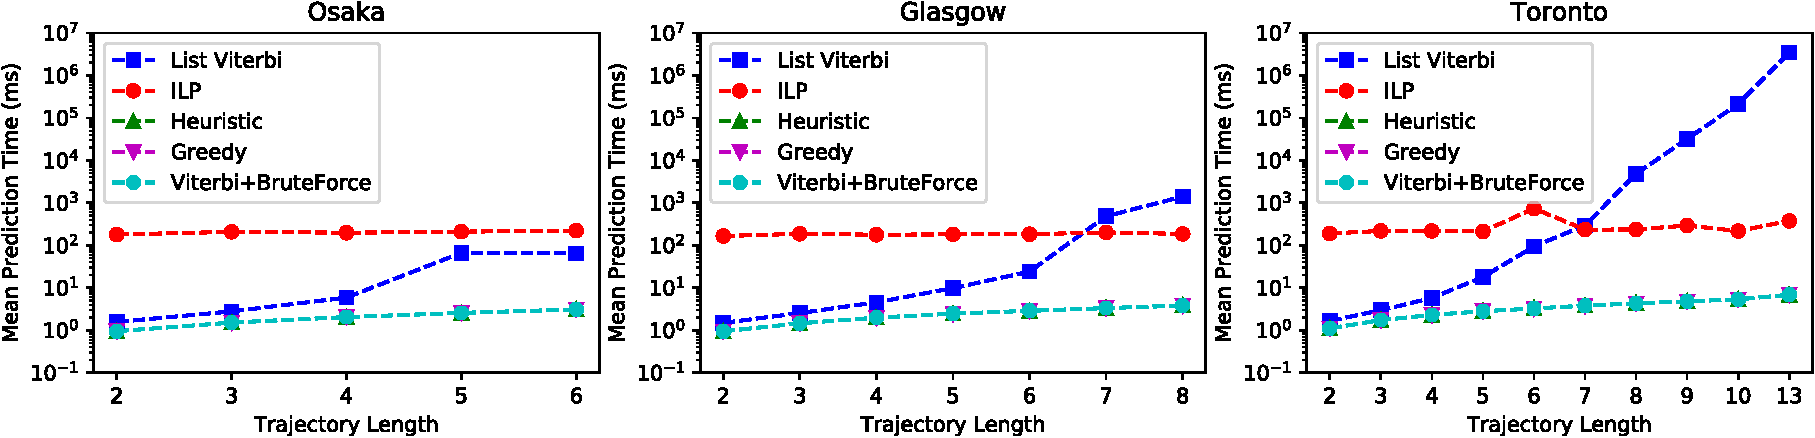
\includegraphics[width=\textwidth]{top1_inftime.pdf}
	    \captionof{figure}{Prediction time for three inference algorithms (in milliseconds)}
	    \label{fig:inftime}
	    %\captionmoveup\eqmoveup
%\end{figure*}%
%\begin{figure*}[!t]
		\quad
		\centering
		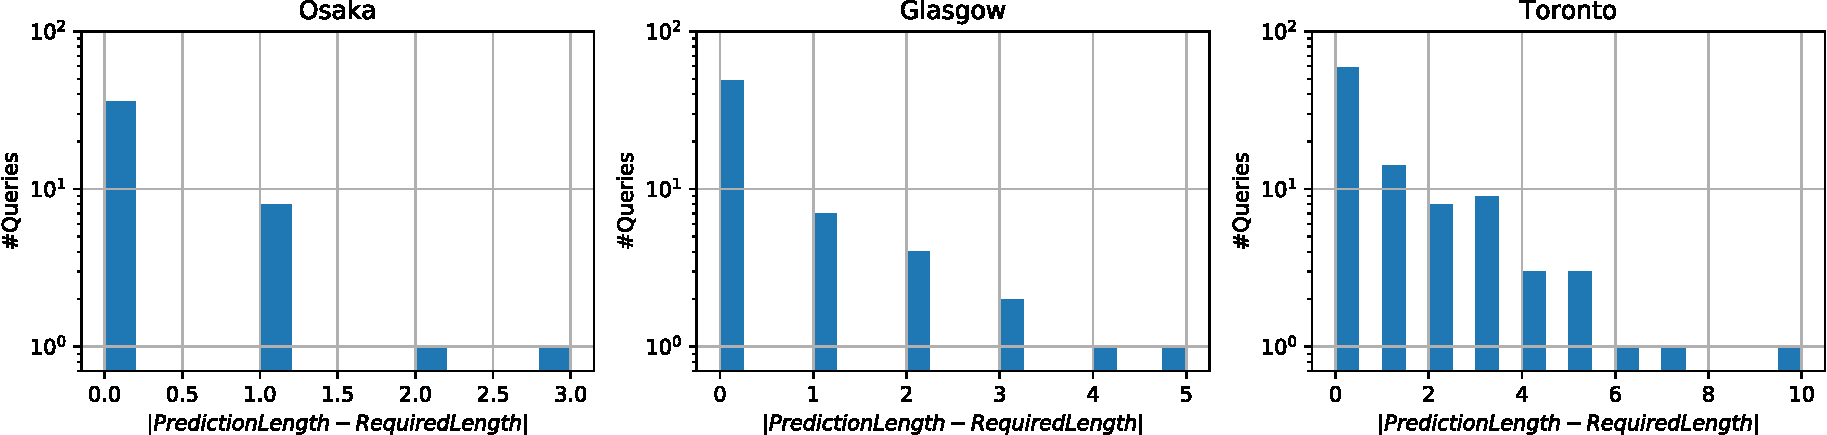
\includegraphics[width=\textwidth]{heu_lengthdiff.pdf}
	    \captionof{figure}{The difference between recommendation and required sequence length.}
	    \label{fig:length-christo}
	    %\captionmoveup\eqmoveup
%\end{figure*}%
%\begin{figure*}[!t]
		\quad
		\centering
		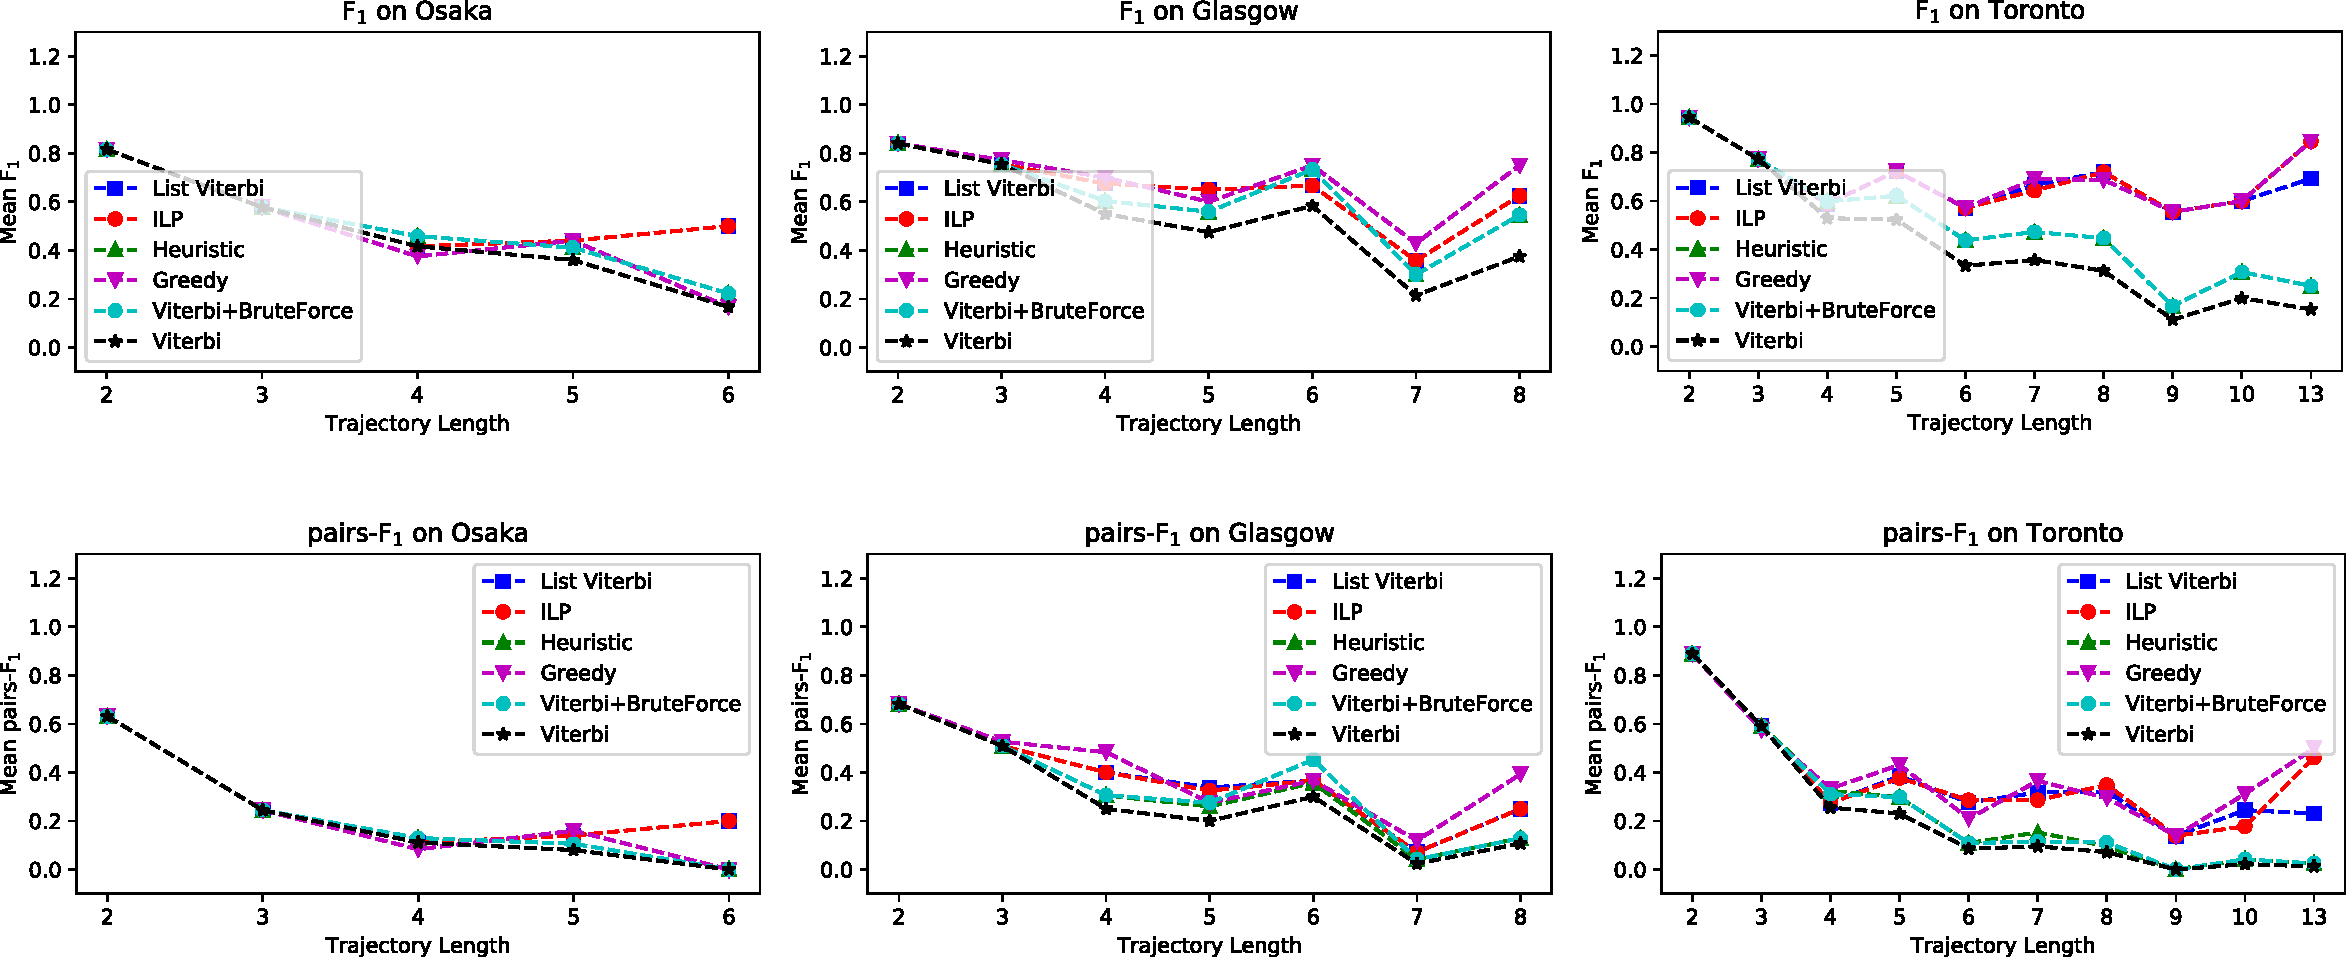
\includegraphics[width=\textwidth]{metrics.pdf}
		% 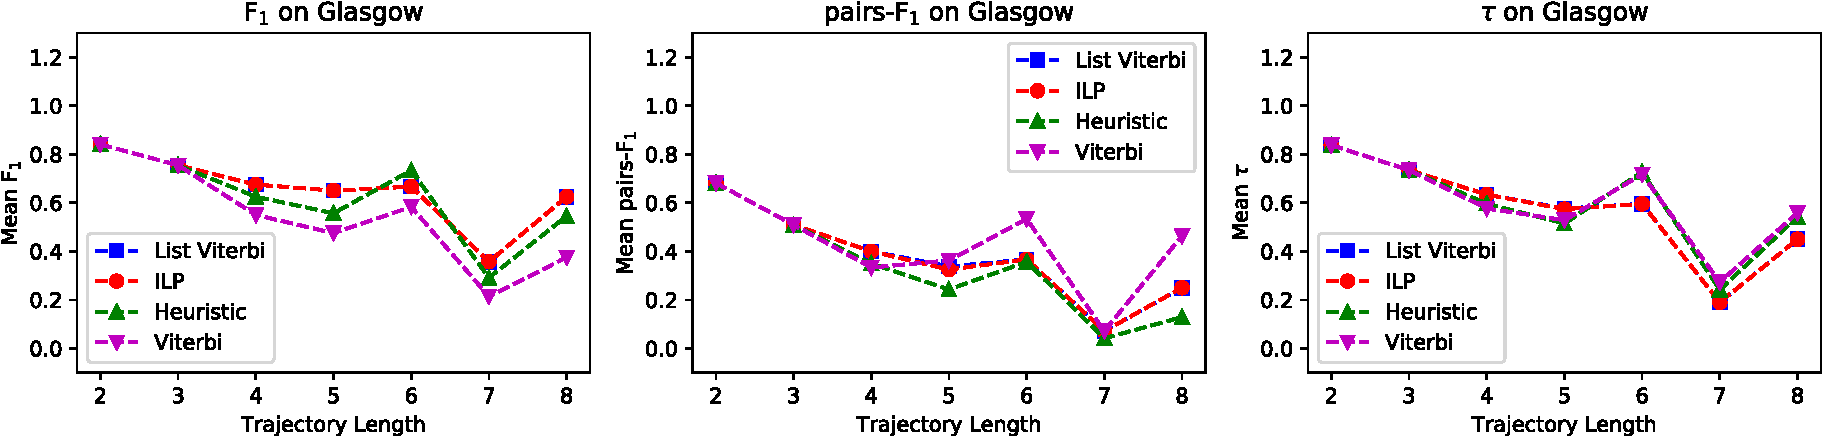
\includegraphics[width=\textwidth]{metric_d2.pdf}
		% 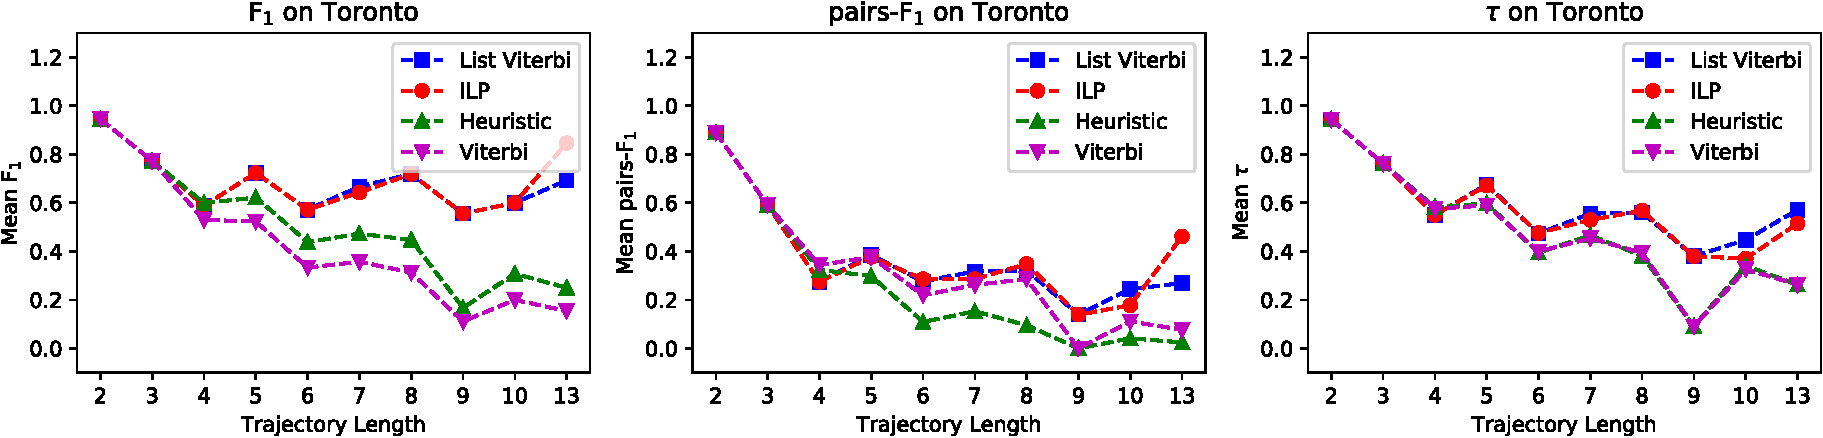
\includegraphics[width=\textwidth]{metric_d3.pdf}
	    \captionof{figure}{Accuracy versus trajectory length.}
	    \label{fig:acc-vs-length}
	    %\captionmoveup\eqmoveup
%\end{figure*}
\end{minipage}
\end{figure*}

% !TEX root=main.tex

{\color{red!75}
\begin{itemize}
	\item Learning
	\item diversity, MMR
	\item See whether any of the workshop topics might have problems that this paper applies.
\end{itemize}
}


\bibliographystyle{ACM-Reference-Format}
\bibliography{ref}

%\clearpage
%\newpage
%\onecolumn
%\appendix
%\section{Notations}

We introduce notations in Table~\ref{tab:symbol_tpush}.
\begin{table}[!h]
\caption{Glossary of commonly used symbols}
\label{tab:symbol_tpush}
\renewcommand{\arraystretch}{1.5} % tweak the space between rows
\setlength{\tabcolsep}{1pt} % tweak the space between columns
\centering
\begin{tabular}{llll}
\toprule
\multicolumn{3}{l}{\textbf{Notation}} & \textbf{Description} \\ \midrule
$D$        &  $\in$  &  $\Z^+$            & The number of features for each song \\
$M$        &  $\in$  &  $\Z^+$            & The number of songs, indexed by $m, n \in \{1,\dots,M\}$ \\
$N$        &  $\in$  &  $\Z^+$            & The number of playlists, indexed by $i \in \{1,\dots,N\}$ \\
$U$        &  $\in$  &  $\Z^+$            & The number of users, indexed by $j \in \{1,\dots,U\}$ \\
$\bv_i$    &  $\in$  &  $\R^D$            & The weights of playlist $i$ \\
$\bu_j$    &  $\in$  &  $\R^D$            & The weights of user $j$ \\
$\widebar\bu$    &  $\in$  &  $\R^D$      & The weights shared by all playlists \\
$\w_i    $ &  $\in$  &  $\R^D$            & The weights for playlist $i$ that owned by user $j=u(i)$, $\w_i = \bv_i + \bu_j + \widebar\bu$ \\
$\Y$       &  $\in$  &  $\R^{M \times N}$ & The matrix of binary labels that indicating if a song is in a playlist \\
$y_m^k$    &  $\in$  &  $\R^D$            & The positive binary label $y_m^k = 1$, \ie song $m$ in playlist $k$ \\
$y_n^k$    &  $\in$  &  $\R^D$            & The negative binary label $y_n^k = 0$, \ie song $n$ not in playlist $k$ \\
$\X$       &  $\in$  &  $\R^{M \times D}$ & The matrix of features of all songs \\
$\x_m$     &  $\in$  &  $\R^D$            & The feature vector of song $m$ \\
$\x_n$     &  $\in$  &  $\R^D$            & The feature vector of song $n$ \\
\bottomrule
\end{tabular}
\end{table}

%\section{Proof of classification objective minimises ranking objective}

The empirical risk $\RCal_\textsc{rank}$ can be approximated (with the exponential surrogate) as follows:
\begin{equation*}
\begin{aligned}
\RCal_\textsc{rank} 
&= \frac{1}{N} \sum_{i=1}^N \frac{1}{M_-^i} \exp \left( -\min_{m: y_m^i = 1} f(i, m) \right) \sum_{n: y_n^i = 0} \exp(f(i, n)) \\
&\approx \frac{1}{N} \sum_{i=1}^N \frac{1}{M_-^i} \exp \left( \frac{1}{p} \log\sum_{m: y_m^i = 1} e^{-p f(i, m)} \right)
         \sum_{n: y_n^i = 0} e^{f(i, n)} \\
&= \frac{1}{N} \sum_{i=1}^N \frac{1}{M_-^i} \exp \left( \log \left( \sum_{m: y_m^i = 1} e^{-p f(i, m)} \right)^\frac{1}{p} \right) 
   \sum_{n: y_n^i = 0} e^{f(i, n)} \\
&= \frac{1}{N} \sum_{i=1}^N \frac{1}{M_-^i} \left( \sum_{m: y_m^i = 1} e^{-p f(i, m)} \right)^\frac{1}{p} \sum_{n: y_n^i = 0} e^{f(i, n)} \\
&= \widetilde\RCal_\textsc{rank}.
\end{aligned}
\end{equation*}

Let $\RCal_\textsc{clf}$ be the following classification risk:
\begin{equation*}
\RCal_\textsc{clf} 
= \frac{1}{N} \sum_{i=1}^N \left( 
  \frac{1}{p M_+^i} \sum_{m: y_m^i = 1} e^{-p f(i, m)} 
  + \frac{1}{M_-^i} \sum_{n: y_n^i = 0} e^{f(i, n)} \right),
\end{equation*}
we have a theorem
\begin{theorem}
Let $\uptheta^* \in \argmin_{\uptheta} \RCal_\textsc{clf}$ (assuming minimisers exist), 
then $\uptheta^* \in \argmin_{\uptheta} \widetilde\RCal_\textsc{rank}$.
\end{theorem}

\begin{proof}
We following the proof technique in~\cite{ertekin2011equivalence}
by first introducing a constant feature $1$ for each song,
without loss of generality, let $x_m^0$ be the constant feature.
Then we can show that
$\frac{\partial \, \RCal_\textsc{clf}} {\partial \, \uptheta} = 0$ implies
$\frac{\partial \, \widetilde\RCal_\textsc{rank}} {\partial \, \uptheta} = 0$,
which means minimisers of $\RCal_\textsc{clf}$ also minimise $\widetilde\RCal_\textsc{rank}$.

First, we introduce a constant feature $1$ for $x_m, \, m \in \{1,\dots,M\}$ to serve as a bias, 
and without loss of generality, let $x_m^0$ be the constant feature, \ie $x_m^0 = 1$, 
$\forall i \in \{1,\dots,N\}$, let
\begin{equation*}
\begin{aligned}
0 
&= \frac{\partial \RCal_\textsc{clf}} {\partial v_i^0}
&= \frac{1}{p M_+^i} \sum_{m: y_m^i = 1} e^{-p f(i, m)} (-p) + \frac{1}{M_-^i} \sum_{n: y_n^i = 0} e^{f(i, n)},
\end{aligned}
\end{equation*}
we have
\begin{equation}
\label{eq:eq1}
\frac{1}{M_+^i} \sum_{m: y_m^i = 1} e^{-p f(i, m)} = \frac{1}{M_-^i} \sum_{n: y_n^i = 0} e^{f(i, n)}.
\end{equation}

Further, let
\begin{equation*}
0 
= \frac{\partial \RCal_\textsc{clf}} {\partial \bv_i} 
= \frac{1}{p M_+^i} \sum_{m: y_m^i = 1} e^{-p f(i, m)} (-p \x_m) + \frac{1}{M_-^i} \sum_{n: y_n^i = 0} e^{f(i, n)} \x_n,
\end{equation*}
we have
\begin{equation}
\label{eq:eq2}
\frac{1}{M_+^i} \sum_{m: y_m^i = 1} e^{-p f(i, m)} \x_m = \frac{1}{M_-^i} \sum_{n: y_n^i = 0} e^{f(i, n)} \x_n.
\end{equation}

Note that
\begin{equation*}
\begin{aligned}
&\frac{\partial \widetilde\RCal_\textsc{rank}} {\partial \bv_i} \\
&= \frac{1}{N M_-^i} \left[ \frac{1}{p} 
   \left( \sum_{m: y_m^i=1} e^{-p f(i, m)} \right)^{\frac{1}{p} - 1} \sum_{m: y_m^i=1} e^{-p f(i, m)} (-p) \x_m \sum_{n: y_n^i=0} e^{f(i, n)}
   + \left( \sum_{m: y_m^i = 1} e^{-p f(i, m)} \right)^\frac{1}{p} \sum_{n: y_n^i = 0} e^{f(i, n)} \x_n \right] \\
&= \frac{-1}{N M_-^i} \left( \sum_{m: y_m^i=1} e^{-p f(i, m)} \right)^{\frac{1}{p} - 1} 
   \left[ \sum_{m: y_m^i=1} e^{-p f(i, m)} \x_m \sum_{n: y_n^i=0} e^{f(i, n)}
   - \sum_{m: y_m^i = 1} e^{-p f(i, m)} \sum_{n: y_n^i = 0} e^{f(i, n)} \x_n \right] \\
&= \frac{-1}{N M_-^i} \left( \sum_{m: y_m^i=1} e^{-p f(i, m)} \right)^{\frac{1}{p} - 1} 
   \left[ \sum_{m: y_m^i=1} e^{-p f(i, m)} \x_m \frac{M_-^i}{M_+^i} \sum_{m: y_m^i=1} e^{-p f(i, m)}
   - \sum_{m: y_m^i = 1} e^{-p f(i, m)} \sum_{n: y_n^i = 0} e^{f(i, n)} \x_n \right] \ \text{(by Eq.~\ref{eq:eq1})} \\
&= \frac{-1}{N M_-^i} \left( \sum_{m: y_m^i=1} e^{-p f(i, m)} \right)^\frac{1}{p} 
   \left[ \frac{M_-^i}{M_+^i} \sum_{m: y_m^i=1} e^{-p f(i, m)} \x_m - \sum_{n: y_n^i = 0} e^{f(i, n)} \x_n \right] \\
&= 0. \ \text{(by Eq.~\ref{eq:eq2})}
\end{aligned}
\end{equation*}

We can similarly prove that 
\begin{equation*}
\begin{aligned}
\frac{\partial \widetilde\RCal_\textsc{rank}}{\partial \bu_j} &= 0, \ \forall j \in \{1,\dots,U\} \\
\frac{\partial \widetilde\RCal_\textsc{rank}}{\partial \widebar{\bu}} &= 0.
\end{aligned}
\end{equation*}

Which means minimisers of $\RCal_\textsc{clf}$ also minimise $\widetilde\RCal_\textsc{rank}$.

\end{proof}



\end{document}
